The CodingInfinity team will be using the \textbf{Agile Software Development methodology} during the course of the project. Agile Software Development is an umbrella term used to refer to the values and principels expressed in the Agile Manifesto.


In particular we find value in the following four points:
\begin{itemize}
	\item \textbf{Individuals and interactions} over processes and tools.
	\item \textbf{Working software} over comprehensive documentation.
	\item \textbf{Customer collaboration} over contract negotiation.
	\item \textbf{Responding to change} over following a plan.
\end{itemize}

Although we find value in the items on the right, we value the items on the left, emphasised in bold, even more.

The Agile princples themselves are derived from the following twelve principles:
\begin{itemize}
  \item Customer satisfaction by early and continuous delivery of valuable software
  \item Welcome changing requirements, even in late development
  \item Working software is delivered frequently (weeks rather than months)
  \item Close, daily cooperation between business people and developers
  \item Projects are built around motivated individuals, who should be trusted
  \item Face-to-face conversation is the best form of communication (co-location)
  \item Working software is the principal measure of progress
  \item Sustainable development, able to maintain a constant pace
  \item Continuous attention to technical excellence and good design
  \item Simplicity—the art of maximizing the amount of work not done—is essential
  \item Best architectures, requirements, and designs emerge from self-organizing teams
  \item Regularly, the team reflects on how to become more effective, and adjusts accordingly
\end{itemize}

Agile development seeks to provide opportunities to assess the changing functional and technical landscape while maintaining focus on rapid and continous delivery of business value. This results in decreased overall risk associated with software development.

A core focus in Agile software development is to ensure that value is continously derived throught the developement lifecycle, which is achieved through a process of continuous planning and feedback. This process creates a feedback loop ensuring that the delivered software can be continuously aligned with the desired business needs and creates the opportunity for easy adaption to changing requirements throughout the process.

With continuous monitoring and measuring of the project status through continuous testing the client gains much more visibility into and around the actual progress of the project.

As a result of following an Agile Development approach the final deliverable software system will be able to much better address the business and customer needs than what would have produced with alternative methodologies.

\begin{figure}[t]
  \centering
  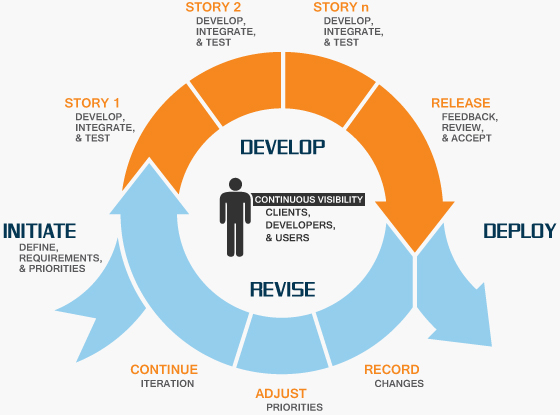
\includegraphics[scale=0.4]{agile.jpg}
  \caption{Agile Development Process}
\end{figure}
